Nedan presenteras resultaten för samtliga mätserier beskrivna i avsnitt \ref{chap:material} i form av figurer och regressionsanalyser. I varje mätserie registrerades drygt 50 mätpunkter där den relativa hastigheten $v_{\text{rel}}$ för ryttarna varierades i det endimensionella fallet och förhållandet mellan puckarnas centrum $d$ enligt ekvation \eqref{ekv:d_calc} i fallet med två dimensioner. Behandling av rådatan görs enligt dataanalys i bilaga \ref{bil:kod} för att få relevanta parametrar till figurerna. 

\subsection{En dimension}
I figur \ref{fig:endimstöt} presenteras mätserier för uppställning \ref{fig:del1}  där $v_{\text{rel}}$ varieras på x-axeln och den beräknade stötkoefficienten från ekvation \eqref{ekv:e} på y-axeln. I figur \ref{fig:estötgummi_bord} användes det gummbiband som visas i figur \ref{fig:del1} som kontaktpunkt vilket visar ett linjärt samband mellan $v_{\text{rel}}$ och $e$. Detta samband visas med hjälp av regressionslinjen $y = -0,24x + 0,89$ som har ett $R^2$-värde på 0,96. Figur \ref{fig:estötmetall} behandlar istället ryttarna utan gummibandet som kontaktpunkt vilket istället visar ett potenssamband enligt  regressionslinjen $y = 0,07x^{-0,42}$ som har ett $R^2$-värde på 0,93.


\begin{figure}[H]
    
    \begin{subfigure}{.5\textwidth}
        \centering
        \hspace*{-1.2cm}
        \includegraphics[width=1\linewidth]{images/estöt_gummi.pdf} %R-squared value: 0.9640957801029384
        \caption{Stötkoefficient beroende på $v_{\text{rel}}$ för ryttare med gummiband som kontaktpunkt.}
        \label{fig:estötgummi_bord}
    \end{subfigure} 
    \hfill
    \hspace*{0.2cm}
    \begin{subfigure}{.5\textwidth}
        \centering
        \hspace*{-1.2cm}
        \includegraphics[width=1\linewidth]{images/estöt_metall.pdf} %R-squared value: 0.9252747767277821
        \caption{Stötkoefficient beroende på $v_{\text{rel}}$ för ryttare med ryttarnas metall som kontaktpunkt.}
        \label{fig:estötmetall}
    \end{subfigure}
    \caption{Stötkoefficienter för kollisioner av ryttare i en dimension. Notera minskningen av $e$ i samband med att $v_{\text{rel}}$ ökar.}
    \label{fig:endimstöt}
\end{figure}

\subsection{Två dimensioner}
I figur \ref{fig:energifördl} visas fördelningen av rotation samt translationsenergi av den totala energin för systemet beroende av $d$, där $d$ är det normerade avståndet mellan masscentran vinkelrät mot hastighetsvektorn i kollisionsögonblicket, enligt uppställningen i figur \ref{fig:del2_bord}.  

\begin{figure}[H]
    \begin{subfigure}{.48\textwidth}
        \centering
        \hspace*{-1.2cm}
        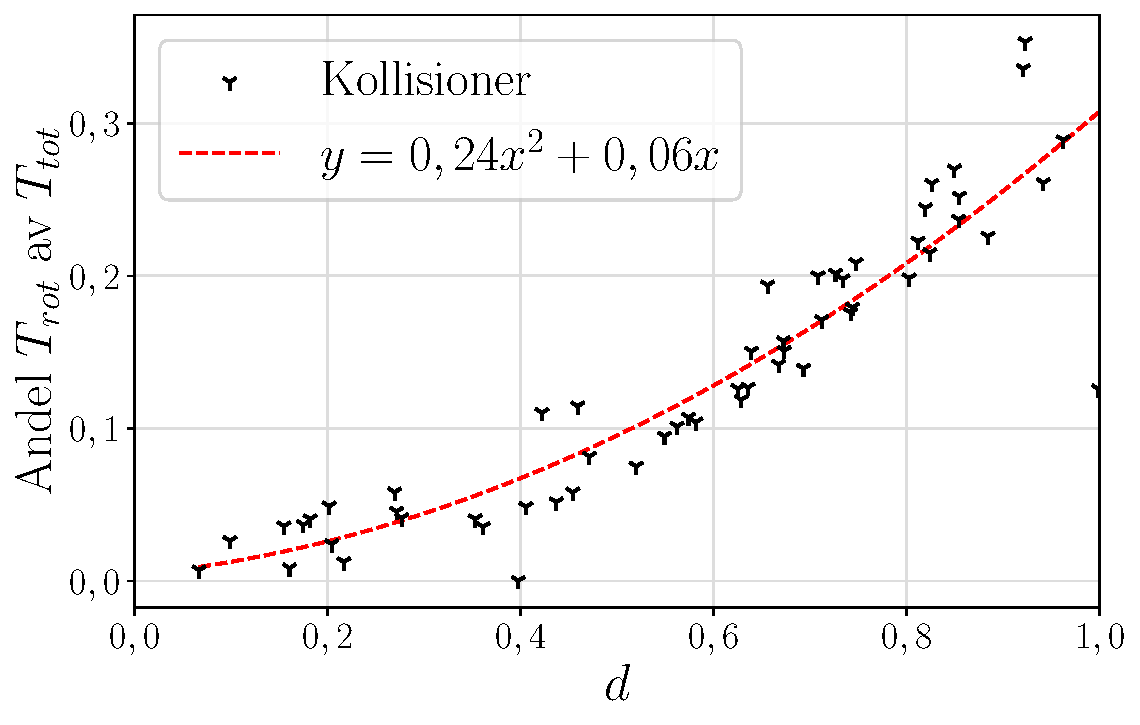
\includegraphics[width=1\linewidth]{images/d_rotationandel.pdf} %R-squared value: 0.8458396030717268
        \caption{Andel rotationsenergi av total energi för kollisioner mellan puckar i två dimensioner beroende på $d$.}
        \label{fig:rot}
    \end{subfigure} 
    \hfill
    \hspace*{0.2cm}
    \begin{subfigure}{.48\textwidth}
        \centering
        \hspace*{-1.2cm}
        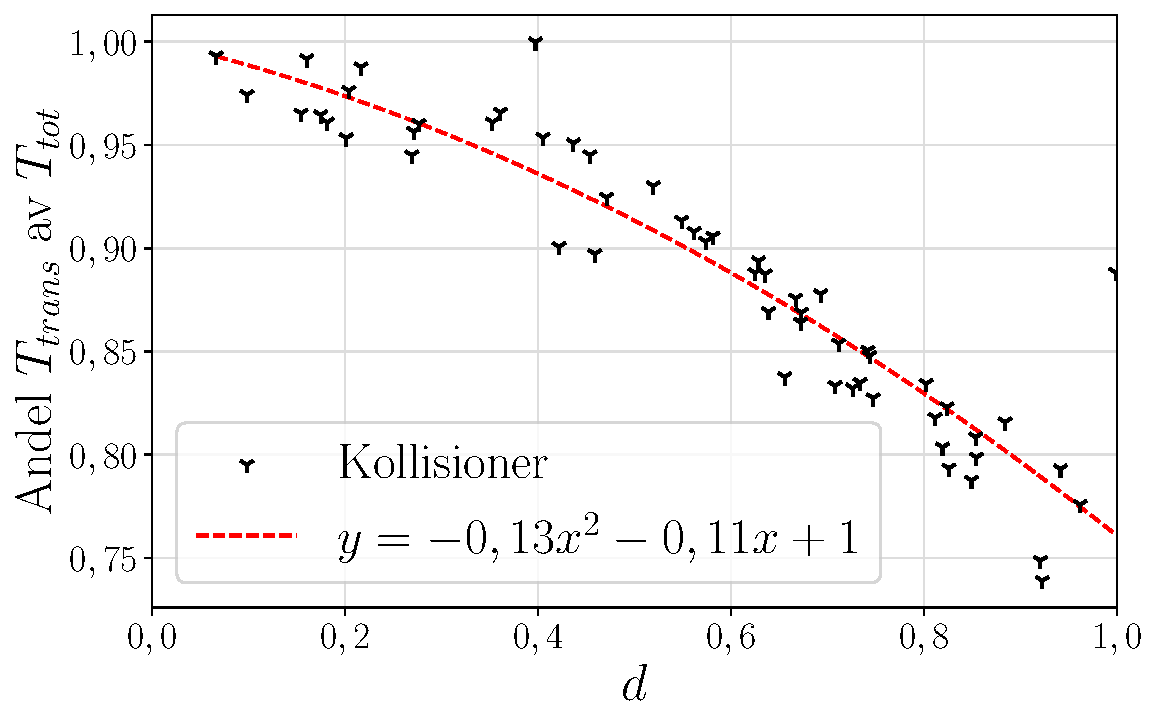
\includegraphics[width=1\linewidth]{images/d_translational_energy_percentage.pdf} %R-squared value: 0.8604999741824243
        \caption{Andel  translationsenergi av total energi för kollisioner mellan puckar i två dimensioner beroende på $d$.}
        \label{fig:trans}
    \end{subfigure}
    \caption{Andel rotations- och translationsenergi för två puckar med avseende på $d$. Notera sambandet mellan rotations- samt translationsenergi och $d$ genom figurernas motsatta trender. Regressionslinjerna har $R^2$-värde på 0,85 respektive 0,86.}
    \label{fig:energifördl}
\end{figure}

Med hjälp av både figur \ref{fig:rot} och figur \ref{fig:trans} syns sambandet att rotationsenergin för systemet ökar i samband med att $d$ ökar och att translationsenergin för systemet ökar när $d$ minskar.

I figur \ref{fig:rörelsemängd} visas rörelsemängden i x'-led och y'-led för puck B med avseende på hastighetsvektorn för puck A som nollställe i ett nydefinerat koordinatsystem med hastighetsvektorn för puck A som utgångspunkt.

\begin{figure}[H]
    
    \begin{subfigure}{.45\textwidth}
        \centering
        \hspace*{-1.2cm}
        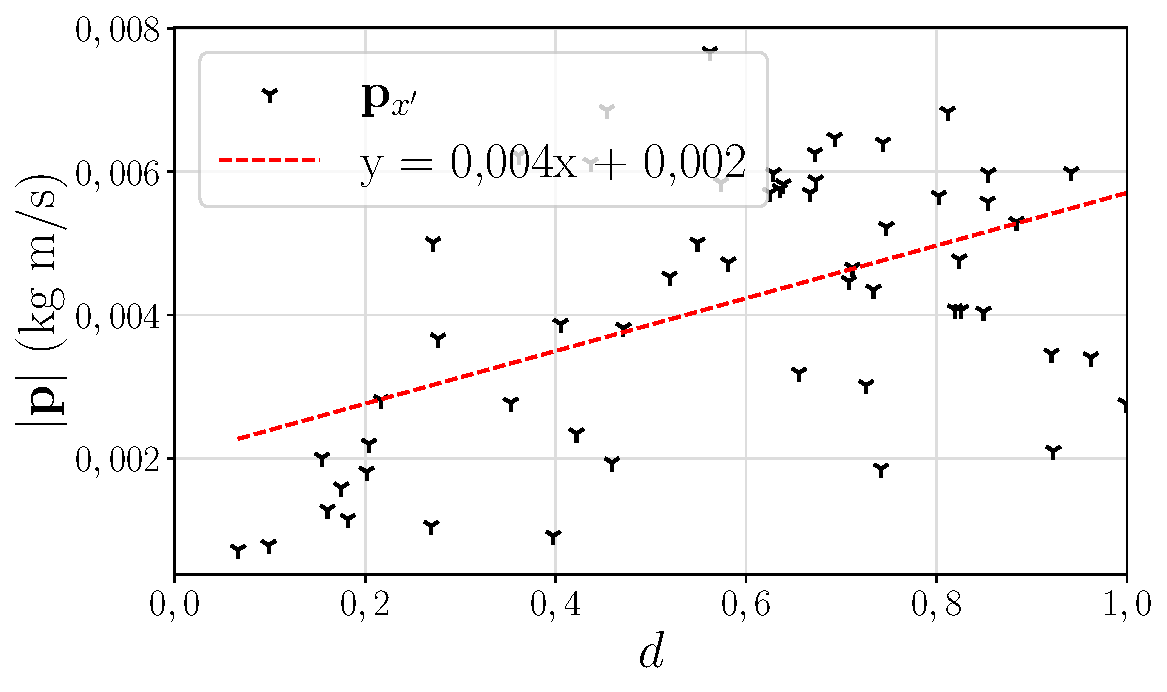
\includegraphics[width=1.2\linewidth]{images/d_pxled.pdf} %R-squared value: 0.2536796041858981
        \caption{Rörelsemängd för puck B i x'-led beroende av $d$. Notera sambandet mellan rörelsemängden och $d$.}
        \label{fig:px}
    \end{subfigure} 
    \hfill
    \begin{subfigure}{.45\textwidth}
        \centering
        \hspace*{-1.2cm}
        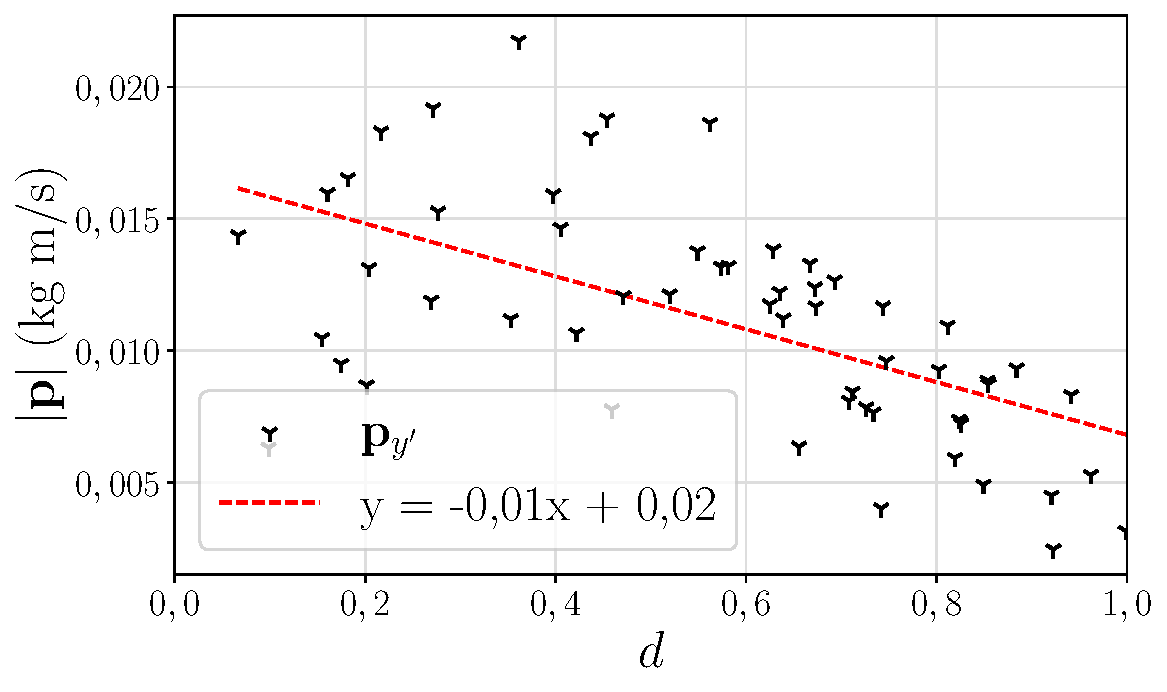
\includegraphics[width=1.2\linewidth]{images/d_pyled.pdf} %R-squared value: 0.34818806187610774
        \caption{Rörelsemängd för puck B i y'-led beroende av $d$. Notera sambandet mellan rörelsemängden och $d$.}
        \label{fig:py}
    \end{subfigure}
    \caption{Rörelsemängdskomposanter beroende av $d$ i ett nydefinerat koordinatsystem med puck A:s hastighetsvektor som utgångspunkt. Notera figurernas motsatta trender. Regressionslinjerna har $R^2$-värde på 0,25 respektive 0,35.}
    \label{fig:rörelsemängd}
\end{figure}
Med hjälp av figur \ref{fig:px} och figur \ref{fig:py} syns sambandet mellan rörelsemängden i x'-led och y'-led i relation till $d$.


I figur \ref{fig:lb-label} visas differensen för den absoluta rörelsemängden för hela systemet före och efter kollision beroende av $d$ där många punkter är centrerade runt 0. I figur \ref{fig:lb-label} visas istället det absoluta rörelsemängdsmomentet för puck B beroende av $d$ där det syns att $\mathbf{L}_b$ ökar i samband med att $d$ ökar. 
 

\begin{figure}[H]
    
    \begin{minipage}{.45\textwidth}
        \centering
        \hspace*{-1.2cm}
        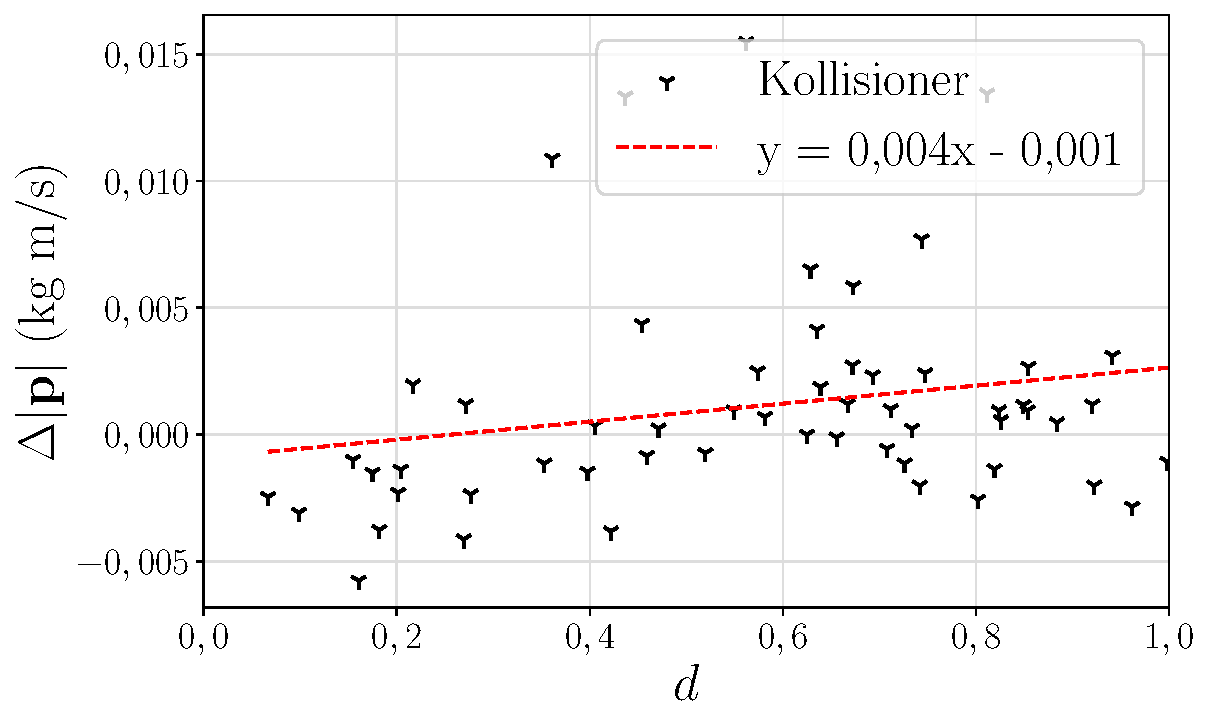
\includegraphics[width=1.2\linewidth]{images/d_deltap2.pdf} %R-squared value: 0.04484322802549928
        \caption{Rörelsemängdsbevaring med avseende på $d$. Notera mätvärdernas centrering kring 0. Regressionlinjen har ett $R^2$-värde på 0,05.}
        \label{fig:rm}
    \end{minipage} 
    \hfill
    \begin{minipage}{.45\textwidth}
        \centering
        \hspace*{-1.2cm}
        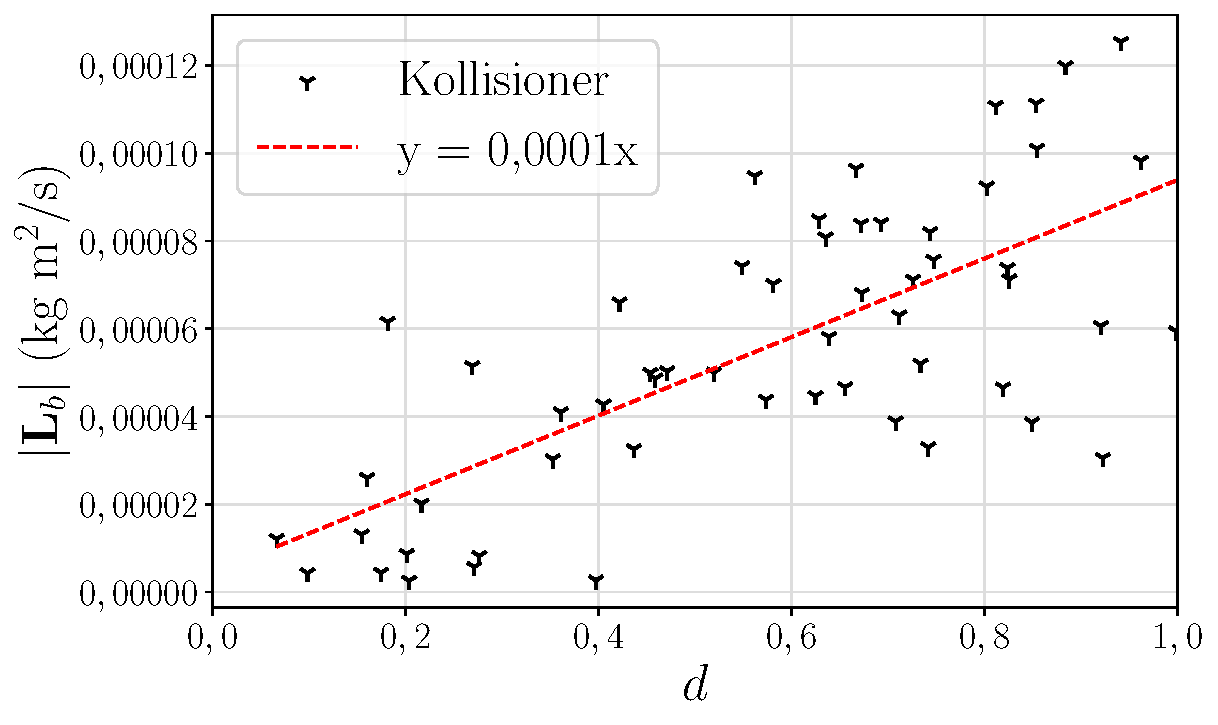
\includegraphics[width=1.2\linewidth]{images/d_lb.pdf} %R-squared value: 0.5087971703532166
        \caption{Rörelsemängdsmomentet för puck B $\mathbf{L}_b$ med avssende på $d$. Notera ökningen av rörelsemängdsmoment när d ökar. Regressionlinjen har ett $R^2$-värde på 0,51. }
        \label{fig:lb-label}
    \end{minipage}
\end{figure}

Felanalysen av resultaten består både av felfortplantningen av mätvärdena, redovisade i bilaga \ref{bil:mätos}, och referensmätningarna av objektens friktion. Referensmätningarna när varje puck och ryttare gled över ytan utan kollision visade att medelvärdet för $\Delta T$ under $\qty{0.4}{s}$ var $\SI{4.8e-4}{J}$ för ryttare A, $\SI{2.9e-4}{J}$ för ryttare B, \( \SI{3.6e-5}{J}\) för puck A och \(\SI{4.2e-5}{J}\) för puck B. 